\documentclass[11pt]{article}
\usepackage{../../tex/math-cmds}
\usepackage{../../tex/analysis}
\usepackage{IEEEtrantools}
\usepackage{mathabx}


\title{Lecture Notes:
A Dataflow Analysis Framework for \textsc{While3Addr}}
\author{17-355/17-665/17-819O: Program Analysis (Spring 2020)\\
        Claire Le Goues\\
		{\tt clegoues@cs.cmu.edu}}
	\date{}



\begin{document}

\maketitle

\section{Defining a dataflow analysis}

A dataflow analysis computes some dataflow information at each program point in
the control flow graph.\footnote{Refer to the first set of course notes for an
  overview of CFGs.} We thus start by examining how this information is 
defined.  We will use $\sigma$ to denote this information. Typically
$\sigma$ tells us something about each variable in the program.  For example,
$\sigma$ may map variables to abstract values taken from some set $L$:

\begin{equation*}
\sigma \in \textit{Var} \rightarrow L
\end{equation*}

$L$ represents the set of abstract values we are interested in tracking in the
analysis.  This varies from one analysis to another.  For example, consider a
\textit{zero analysis}, which tracks whether each variable is zero or not at
each program point (Thought Question: Why would this be useful?).  For this
analysis, we define $L$ to be the set $\{Z, N, \top \}$.  The abstract value $Z$
represents the value 0, $N$ represents all nonzero values.  $\top$ is pronounced
``top'', and we define it more concretely later it in these notes; we use it as
a question mark, for the situations when we do not know whether a variable is
zero or not, due to imprecision in the analysis.

Conceptually, each abstract value represents a set of one or more concrete
values that may occur when a program executes.  We define an abstraction function $\alpha$ that maps each
possible concrete value of interest to an abstract value:

\begin{equation*}
\alpha : \Integer \rightarrow L
\end{equation*}

\noindent For zero analysis, we define $\alpha$ so that 0 maps to $Z$ and
all other integers map to $N$:


\begin{IEEEeqnarray*}{ll}
\alpha_Z(0) = Z \\
\alpha_Z(n) = N & \mbox{where}~ n \neq 0
\end{IEEEeqnarray*}

%Consider the gains we achieve despite the loss of precision: instead of tracking
%$2^{64}$ possible concrete values per variable (assuming 64-bit integers), we're
%only tracking 3 possible abstract values!

The core of any program analysis is how individual instructions in the program
are analyzed and affect the analysis state $\sigma$ at each program point. We
define this using \textit{flow functions} that map the dataflow information at
the program point immediately \emph{before} an instruction to the dataflow
information \emph{after} that instruction.  A flow function should represent the
semantics of the instruction, but abstractly, in terms of the abstract values
tracked by the analysis. We will link semantics to the flow function
precisely when we talk about correctness of dataflow analysis.  For now, to
approach the idea by example, we define the flow functions $f_Z$ for zero
analysis on \WhileThAddr as follows:

\begin{IEEEeqnarray}{lcl}
f_Z\parg{x := 0}(\sigma) & = [x \mapsto Z]\sigma \\
f_Z\parg{x := n}(\sigma) & = [x \mapsto N]\sigma & \mbox{where}~ n \neq 0\\[1ex]
f_Z\parg{x := y}(\sigma) & = [x \mapsto \sigma(y)]\sigma\\[1ex]
f_Z\parg{x := y ~op~ z}(\sigma) & = [x \mapsto \top]\sigma\\[1ex]
f_Z\parg{\mbox{goto}~n}(\sigma) & = \sigma\\[1ex]
f_Z\parg{\mbox{if}~x=0~\mbox{goto}~n}(\sigma) & = \sigma
\end{IEEEeqnarray}

In the notation, the form of the instruction is an implicit argument to the
function, which is followed by the explicit dataflow information argument, in
the form $f_Z\parg{I}(\sigma)$.  (1) and (2) are for
assignment to a constant.  If we assign 0 to a variable $x$, then we should
update the input dataflow information $\sigma$ so that $x$ maps to the abstract
value $Z$.  The notation $[x \mapsto Z]\sigma$ denotes dataflow information that
is identical to $\sigma$ except that the value in the mapping for $x$ is updated
to refer to $Z$.
%
Flow function (3) is for copies from a variable $y$ to another variable
$x$:  we look up $y$ in
$\sigma$, written $\sigma(y)$, and update $\sigma$ so that $x$ maps to the same
abstract value as $y$.

We start with a generic flow function for arithmetic instructions (4).  
Arithmetic can produce either a zero or a nonzero value, so we use
the abstract value $\top$ to represent our uncertainty.  More precise flow
functions are available based on certain instructions or operands.  For example, if the instruction is
subtraction and the operands are the same, the result will definitely be zero.  Or,
if the instruction is addition, and the analysis information tells us that one
operand is zero, then the addition is really a copy and we
can use a flow function similar to the copy instruction above.  These examples
could be written as follows (we would still need the generic case above for
instructions that do not fit such special cases):

\[
\begin{array}{lll}

f_Z\parg{x := y - y}(\sigma) & = [x \mapsto Z]\sigma\\[1ex]
f_Z\parg{x := y + z}(\sigma) & = [x \mapsto \sigma(y)]\sigma & \mbox{where}~ \sigma(z)=Z\\[1ex]

\end{array}
\]

\exercise{1} Define another flow function for some arithmetic instruction and
certain conditions where you can also provide a more precise result than $\top$.

\answer{1}{We can define the following flow function for multiplication by
  zero:\\ \[f_Z\parg{x := y * z}(\sigma) = [x \mapsto Z]\sigma ~~~~
  \mbox{where}~ \sigma(y)=Z \lor \sigma(z)=Z \]}

The flow function for branches ((5) and (6)) is trivial:  branches do not change the
state of the machine other than to change the program counter, and thus the analysis result is unaffected.

However, we can provide a better flow function for conditional branches if we
distinguish the analysis information produced when the branch is taken or not
taken.  To do this, we extend our notation once more in defining flow functions
for branches, using a subscript to the instruction to indicate whether we are
specifying the dataflow information for the case where the condition is true
($T$) or when it is false ($F$).  For example, to define the flow function for
the true condition when testing a variable for equality with zero, we use the
notation $f_Z\parg{\mbox{if}~x=0~\mbox{goto}~n}_T(\sigma)$.  In this case we
know that $x$ is zero so we can update $\sigma$ with the $Z$ lattice value.
Conversely, in the false condition we know that $x$ is nonzero:

\[
\begin{array}{lll}

f_Z\parg{\mbox{if}~x=0~\mbox{goto}~n}_T(\sigma) & = [x \mapsto Z]\sigma\\
f_Z\parg{\mbox{if}~x=0~\mbox{goto}~n}_F(\sigma) & = [x \mapsto N]\sigma\\[1ex]

\end{array}
\]

\exercise{2}  Define a flow function for a conditional branch testing whether a variable $x < 0$.

\answer{2}{We get no additional information in the false case.  However, we can define the true case as follows:\\ \[ f_Z\parg{\mbox{if}~x<0~\mbox{goto}~n}_T(\sigma) = [x \mapsto N]\sigma \]}

\section{Running a dataflow analysis}

The point of developing a dataflow analysis is to compute information about
possible program states at each point in a program.  For example, for
of zero analysis, whenever we divide some expression by a variable $x$, we might
like to know whether $x$ must be zero (the abstract value $Z$) or
may be zero (represented by $\top$) so that we can warn the developer.

\subsection{Straightline code}

One way to think of a simple dataflow analysis is that are statically simulating
program execution, tracking only the information we care about.  For each node in the CFG (each of which contains an
instruction), we use the flow function to compute the dataflow analysis
information at the program point immediately \emph{after} that node
from the information we had at the program point \emph{before} that node.
To demonstrate, consider the following simple program (left), with its control flow graph (middle):

% close your eyes
\begin{center}
\begin{minipage}[t][-9.7em][b]{0.30\textwidth} % toggle vertical alignment of table
 $\begin{array}{ll}
 1: & x := 0\\
 2: & y := 1\\
 3: & z := y\\
 4: & y := z + x\\
 5: & x := y - z\\
\end{array}$
\end{minipage}
\hspace*{1em}% \hspace whatever for space between
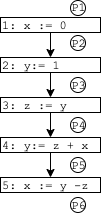
\includegraphics[scale=0.75]{images/df-notes-cfg}
\hspace*{3em}
\begin{minipage}[t][-9.7em][b]{0.30\textwidth} % toggle vertical alignment of table
\begin{tabular}{r | c c c}
  & x & y & z \\
\hline
P1 & ? & ? & ? \\
P2 & Z & ?  & ? \\
P3 & Z & N & ? \\
P4 & Z & N & N\\
P5 & Z & N & N\\
P6 & $\top$ & N & N\\
\end{tabular}
\end{minipage}
\end{center}
% ok you can open them again

For such simple code, we can track analysis information using a table with a
column for each program variable and a row for each program point (right,
above). 

The first thing to notice is that, because flow functions operate on the
abstract state for the program point immediately before a node, we need some
kind of \emph{initial} assumption (this confusion is illustrated by the ? in
the cells of the table).  We will return to this point in a moment, since those
values don't influence the analysis for such simple, straight-line code. 

Notice also that the analysis is imprecise at the end with respect to the value of
$x$.  We were able to keep track of which values are zero and nonzero quite well
through instruction 4, using (in the last case) the flow function that knows
that adding a variable known to be zero is equivalent to a copy.
However, at instruction 5, the analysis does not know that $y$ and $z$ are
equal, and so it cannot determine whether $x$ will be zero.  Because the
analysis is not tracking the exact values of variables, but rather
approximations, it will inevitably be imprecise in certain situations.  However,
in practice, well-designed approximations can often allow dataflow analysis to
compute quite useful information.


\subsection{Alternative Paths: Illustration}
\label{sec:if}

Things get more interesting in \WhileThAddr code that contains \texttt{if}
statements.  An \texttt{if} statement introduces two possible paths through the
program. 
Consider the following simple example (left), and its CFG (middle).\footnote{A
  point on diagrams: in the interest of clarity, we sometimes
elide program points between nodes when we can. That is, in this example,,
the state going into instruction 3 is exactly the state coming out of
instruction 2, so we label a single program point P3.  However, when we need to
consider multiple paths to determine the incoming state at a node, we often need
differentiate the two program points in our CFG diagrams.}
  We will
begin by analyzing the first node as though the branch is not taken:

\begin{center}
\begin{minipage}[t][-9.7em][b]{0.3\textwidth} % toggle vertical alignment of table
\[
\begin{array}{ll}
1: & \mbox{if}~x=0~\mbox{goto}~4\\
2: & y := 0\\
3: & \mbox{goto}~6\\
4: & y := 1\\
5: & x := 1\\
6: & z := y\\
\end{array}
\]
\end{minipage}
%\hspace*{1em}% \hspace whatever for space between
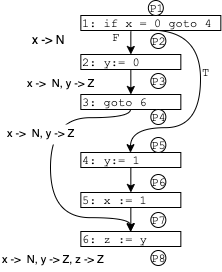
\includegraphics[scale=0.75]{images/df-notes-if1}
%\hspace*{1em}
\begin{minipage}[t][-9.7em][b]{0.30\textwidth} % toggle vertical alignment of table
\begin{tabular}{r | c c c}
  & x & y & z \\
\midrule
P1 & ?  & ?  & ? \\
P2 & $N_F$ & ? & ?  \\
P3 & N & Z & ?  \\
P4 & N & Z & ? \\
P5 &   &   &  \\
P6 &   &   &  \\
P7 & N?  & Z?   & ??  \\
P8 & N?? & Z?? & Z?? \\
\end{tabular}
\end{minipage}
\end{center}
% ok you can open them again

In the table above, the entry for $x$ at P2 indicates the abstract value
produced for the false condition on the branch, which is then used as input to
analyze instruction 2 (and produce the state at P3). We can go right from P3 to
P4 without any complexity.
%
But, if we just continue ``simulating'' execution, we get to P7.  It has \emph{two}
possible incoming edges, so two possible incoming states to use for the flow
function for instruction 6.  What to do?
We have not yet analyzed a path through lines 4 and 5.  The table shows the
(questionable) values if we just use the state coming from P4 as ``incoming'' at
instruction 6, and ignore what might have happened along that other path. 

Perhaps turning to that alternative path, will give answers.  
Let's analyze instructions 4 and 5 as if we had taken the
true branch at instruction 1:

\tablespace
\begin{center}
\begin{minipage}[t][-9.7em][b]{0.5\textwidth} % toggle vertical alignment of table
\begin{tabular}{r | c c c l}
  & x & y & z \\
\hline
P1 & ? & ?   & ?  \\
P2 & $Z_T,N_F$ & ?  & ?  \\
P3 & N & Z & ?  \\
P4 & N & Z & ?  \\
P5 & Z & ? & ?  \\
P6 & Z & N & ? &   \\
P7 & N & N? & ? & \textit{note: different!} \\
P8 & N?? & N?? & N?? & \textit{??????} \\
\end{tabular}
\end{minipage}
\hspace*{1em}% \hspace whatever for space between
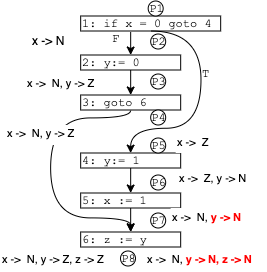
\includegraphics[scale=0.8]{images/alternativepathwrong}
\end{center}
\tablespace

We have a dilemma.  The first time we analyzed instruction 6, the incoming state
had come from instruction 3, where $x$ was nonzero and $y$ was zero.  Now have,
the incoming state coming from instruction 5 is different:  $x$ is still nonzero,
but so is $y$!

We resolve this dilemma by \emph{combining} the abstract values computed along the two
paths for $y$. The incoming abstract values at P7 for $y$ are $N$
and $Z$.    We represent this uncertainty
with a new abstract
value $\top$ (pronounced ``top'').  This value indicates that we do know know if $y$ is zero or not,
because we don't know how we reached this program location. 
We can apply similar logic to $x$, but because $x$ is
nonzero on both incoming paths, we can maintain our knowledge that $x$ is
nonzero.  Thus, we should analyze instruction 6 with this combined
incoming state:  $\{x \mapsto N, y \mapsto {\top}\}$.  

The corrected analysis, showing the \emph{combined} state at P6, looks like: 

\tablespace
\begin{center}
\begin{minipage}[t][-9.7em][b]{0.5\textwidth} % toggle vertical alignment of table
\begin{tabular}{r | c c c l}
  & x & y & z \\
\hline
P1 & ? & ? & ? \\
P2 & $Z_T,N_F$ & ?  & ? \\
P3 & N & Z & ? \\
P4 & N & Z & ? \\
P5 & Z & ? & ?  \\
P6 & Z & N & ?  \\
P7 & N & $\top$ & ? & \textit{combined with P4} \\
P8 & N & $\top$ & $\top$ & \textit{corrected}\\
\end{tabular}
\end{minipage}
\hspace*{1em}
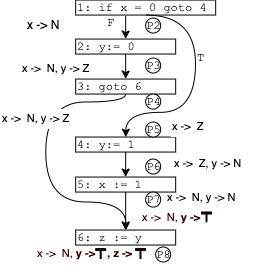
\includegraphics[scale=0.8]{images/altpathright}
\end{center}
\tablespace

\section{Join}

The mechanism for combining analysis results along multiple paths
is called a \emph{join} operation, $\join$.  When taking two abstract values $l_1, l_2
\in L$, the result of $l_1 \join l_2$ is an abstract value $l_j$ that
generalizes both $l_1$ and $l_2$.

To precisely define what ``generalizes'' means, we define a partial order $\alap$
over abstract values, and say that $l_1$ and $l_2$ are at least as precise as
$l_j$, written $l_1 \alap l_j$.  Recall that a partial order is any relation
that is:

\begin{itemize}[labelwidth=0.7em, labelsep=0.6em, topsep=0ex, itemsep=0ex,
  parsep=0ex]
\item reflexive: $\forall l : l \alap l$
\item transitive: $\forall l_1, l_2, l_3 : l_1 \alap l_2 \land l_2 \alap l_3 \implies l_1 \alap l_3$
\item anti-symmetric: $\forall l_1, l_2 : l_1 \alap l_2 \land l_2 \alap l_1 \implies l_1 = l_2$
\end{itemize}

A set of values $L$ that is equipped with a partial order $\alap$, and for which
the least upper bound of any two values in that ordering $l_1 \join l_2$ is
unique and is also in $L$, is called a \textit{join-semilattice}.  Any
join-semilattice has a maximal element $\top$ (pronounced ``top'').  We require
that the abstract values used in dataflow analyses form a join-semilattice.  We
will use the term lattice for short; as we will see below, this is the correct
terminology for most dataflow analyses anyway.
%
For zero analysis, we define the partial order with $Z \alap \top$ and $N \alap
\top $, where $Z \join N = \top$.


We have now considered all the elements necessary to define a
dataflow analysis:

\begin{itemize}[labelwidth=0.7em, labelsep=0.6em, topsep=0ex, itemsep=0ex,
  parsep=0ex]
\item a lattice $(L,\alap)$
\item an abstraction function $\alpha$
\item a flow function $f$
\item initial dataflow analysis assumptions, $\sigma_0$
\end{itemize}

Note that the theory of lattices answers that side question that came up in the
very first example: what should we assume
about the value of input variables (the question marks in our example tables)? 
If we do not know anything about the value $x$ can be,
one good choice is to assume it can be anything. That is, in the initial
environment $\sigma_0$, variables' initial state is mapped to $\top$.  

\subsection{Dataflow analysis of loops}

We now consider \textsc{While3Addr} programs with loops. Our intuition above,
which simply analyzed the two paths induced by the \texttt{if} statement
separately, no longer works so well.  A loop produces a potentially unbounded
number of program paths, and we want our analysis to take only bounded
time. Consider the following simple
looping example:\footnote{I provide the CFG for reference but omit the
  annotations in the interest of a cleaner diagram.  Notice that I differentiate
  P2 and P3 because of the join, as well as P7 and P8,
  since they don't both come from instruction 6.}

\tablespace
\begin{center}
\begin{minipage}[t][-9.7em][b]{0.3\textwidth} % toggle vertical alignment of table
%\begin{tabular}{l@{\hskip 0.5in}|@{\hskip 0.5in}l}
$\begin{array}{ll}
1: & x := 10\\
2: & y := 0\\
3: & \mbox{if}~x=0~\mbox{goto}~7\\
4: & y := 1\\
5: & x := x - 1\\
6: & \mbox{goto}~3\\
7: & x := y\\
\end{array}$
\end{minipage}
%\hspace*{1em}
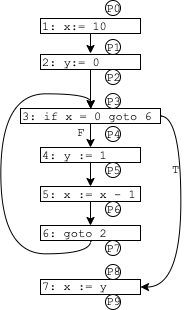
\includegraphics[scale=0.8]{images/loop}
%\hspace*{1em}
\begin{minipage}[t][-9.7em][b]{0.3\textwidth} % toggle vertical alignment of table
\begin{tabular}{r | c c l}
  & x & y  \\
\hline
P0 & $\top$ & $\top$   \\
P1 & N & $\top$   \\
P2 & N & Z  &   \\
P3 & N & Z  & \textit{first time through...}   \\
P4 & $N_F$ & Z  \\
P5 & N & N \\
P6 & $\top$ & N \\
P7 & $\top$ & N \\
P8 & $Z_t$ & N  & \textit{first time through...}  \\
P9 & N  & N &  \textit{first time through...}   \\
\end{tabular}
\end{minipage}
\end{center}
\tablespace

The right-hand side above shows the straightforward straight-line analysis of the path that runs
the loop exactly once.  Thinking back to our handling of \texttt{if} above, we might now
reconsider instruction 3, joining the states at P2 and P7 to create a new
P3. For x, $N \join \top = \top$.  For y, $Z \join N = \top$.
%
This changes the incoming values at instruction 3. 
We can now choose between two paths once again.  We will choose (arbitrarily, for now) to stay
within the loop, and reconsider instruction 4.  We have new incoming information
(at P4, where
both $x$ and $y$ are now $\top$).  But, since instruction 4 assigns $1$ to
$y$, we still know that $y$ is nonzero at P5. The updated input data does not
change the analysis results at P5.

A quick check shows that going through the remaining instructions in the loop,
even back to instruction 3, the analysis information will no longer change.
That is because the flow functions are deterministic: given the same input
analysis information and the same instruction, they will produce the same output
analysis information.  

We say that the dataflow analysis has reached a \textit{fixed
  point} (or fixpoint).  In
mathematics, a fixed point of a function is a data value $v$ that is mapped to
itself by the function, i.e., $f(v) = v$.  In analysis, the mathematical
function is the flow function, and the fixed point is a tuple of the dataflow
analysis values at each program point.  If
we invoke the flow function on the fixed point, the analysis results do not
change (we get the same fixed point back).

Once we have reached a fixed point for the loop,
further analysis of the loop will not be useful.  Therefore, we will
proceed to analyze statement 7.  The final analysis results are as follows:

\tablespace
\begin{center}
\begin{tabular}{r | c c l}

  & x & y & \\
\hline
P0 & $\top$ & $\top$ & \\
P1 & N & $\top$ & \\
P2 & N & Z  &   \\
P3 & $\top$ & $\top$ &  \textit{join} \\
P4 & $N_F$ & $\top$ & \textit{updated} \\
P5 & N & N & \textit{already at fixed point} \\
P6 & $\top$ & N &  \textit{already at fixed point} \\
P7 & $\top$ & N & \textit{already at fixed point} \\
P8 & $Z_T$ & $\top$ &  \textit{updated}  \\
P9 & $\top$ & $\top$ &  \textit{updated}  \\
\end{tabular}
\end{center}
\tablespace

Quickly simulating a run of the program program shows that these results
correctly approximate actual execution.  The uncertainty in the value of $x$ at
P6 and P7 is real: $x$ \emph{is} nonzero after these instructions, except
the last time through the loop, when it is zero.  The uncertainty in the value
of $y$ at the end shows analysis imprecision: this loop
always executes at least once, so $y$ will be nonzero at these points.  However, the analysis
(as currently formulated) cannot tell this for certain, 
so it reports that it cannot tell if $y$ is zero or not.  This is
safe---it is always correct to say the analysis is uncertain---but not as
precise as would be ideal.

The benefit of analysis, however, is that we can gain correct information about
all possible executions of the program with only a finite amount of work.  In
our example, we only had to analyze the loop statements at most twice each
before reaching a fixed point. This is a significant improvement over the actual
program execution, which runs the loop 10
times.  We sacrificed precision in exchange for
coverage of all possible executions, a classic tradeoff.

How can we be confident that the results of the analysis are correct, besides
simulating every possible run of a (possibly very complex) program? The
intuition behind correctness is the invariant that at each program point, the
analysis results approximate all the possible program values that could exist at
that point.  If the analysis information at the beginning of the program
correctly approximates the program arguments, then the invariant is true at the
beginning of program execution.  One can then make an inductive argument that
the invariant is preserved.  In particular, when the
program executes an instruction, the instruction modifies the program's state.
As long as the flow functions account for every possible way that instruction
can modify state, then at the analysis fixed point they will have
correctly approximated actual program execution. 
We will make this argument more precise in a future lecture.


\subsection{A convenience: the $\bottom$ abstract value and complete lattices}

To define an algorithm for dataflow anlaysis more precisely, we need to be more
concrete about how to compute incoming states for CFG nodes with multiple
incoming edges (like instruction 3, above).  We've been ignoring these in our
``one path at a time'' approach so far, but this is a handwave for didactic
purposes. 

Instead, it is more precise and consistent to say that analyzing an instruction \emph{always} uses the
incoming dataflow analysis information from \emph{all} instructions that could precede
it.  However, for instruction 3, this requires a dataflow value from
instruction 6, even if instruction 6 has not yet been analyzed.  We
could do this if we had a dataflow value that is always ignored when it is
joined with any other dataflow value.  In other words, we need a abstract
dataflow value $\bottom$ (pronounced ``bottom'') such that $\bottom \join l =
l$.

$\bottom$ plays a dual role to the value $\top$: it sits at the bottom of the
dataflow value lattice.  For all $l$, we have the identity $l \alap \top$ and
correspondingly $\bottom \alap l$.  There is an greatest lower bound operator
\textit{meet}, $\meet$, which is dual to $\join$.  The meet of all dataflow
values is $\bottom$.

A set of values $L$ that is equipped with a partial order $\alap$, and for which
both least upper bounds $\join$ and greatest lower bounds $\meet$ exist in $L$
and are unique, is called a \emph{complete lattice}.

This provides an elegant solution to
the problem mentioned above.  We initialize $\sigma$ at every program point in
the program, except at entry, to $\bottom$, indicating that the instruction
there has not yet been analyzed.  We can then \emph{always} merge all input
values to a node, whether or not the sources of those inputs have been analysed,
because we know that any $\bottom$ values from unanalyzed sources will simply be
ignored by the join operator $\join$, and that if the dataflow value for that
variable will change, we will get to it before the analysis is completed.

\section{Analysis execution strategy}


\definecolor{dkgreen}{rgb}{0,0.5,0}
\definecolor{dkred}{rgb}{0.5,0,0}
\definecolor{gray}{rgb}{0.5,0.5,0.5}

\lstdefinestyle{javastyle} {
language=Java,
basicstyle=\ttfamily,
  morekeywords={virtualinvoke},
  keywordstyle=\color{blue},
  ndkeywordstyle=\color{red},
  commentstyle=\color{dkred},
  stringstyle=\color{dkgreen},
  numbers=none,
  breaklines=true,
  numberstyle=\ttfamily\footnotesize\color{gray},
  stepnumber=1,
  numbersep=10pt,
  backgroundcolor=\color{white},
  tabsize=4,
  showspaces=false,
  showstringspaces=false,
%  xleftmargin=.23in
}
\lstset{style=javastyle}


Our informal strategy above, which considers all paths until the dataflow
analysis information reaches a fixed point, can be simplified.  The argument for
correctness outlined above implies that for correct flow functions, it doesn't
matter how we get to the analysis fixed point (it would be
surprising if analysis correctness depended on which branch of an \texttt{if} statement
we explored first!).  It is in fact possible to run the analysis on program
instructions in any order we choose.  As long as we continue doing so until a
reaching a fixed point, the final result will be correct.  The simplest
correct algorithm for executing dataflow analysis can therefore be stated as
follows:

\begin{lstlisting}[mathescape]
for Node n in cfg
    results[n] = $\bottom$
results[0] = initialDataflowInformation

while not at fixed point
    pick a node n in program
	input = join { results[j] | j in predecessors(n) }
	output = flow(n, input)
	results[n] = output
\end{lstlisting}

Or, equivalently:

\begin{lstlisting}[mathescape]
for Node n in cfg
    input[n] = $\bottom$
input[0] = initialDataflowInformation

while not at fixed point
    pick a node n in program
    output = flow(n, input[n])
    for Node j in sucessors(n)
        input[j] = input[j] $\join$ output
\end{lstlisting}

In the code above, the termination condition is expressed abstractly (``not at
fixed point'').  It can easily be checked by keeping track, when we process each
node, whether the new results have changed compared to what we previously
had stored for that node.  If the results do not change for any node, the
analysis has reached a fix point. 

How do we know the algorithm will terminate?  The intuition is as follows.  We
rely on the choice of a node to be fair, so that each node is
eventually considered.  As long as the analysis is not at a fixed point, some
node can be analyzed to produce new results.  If our flow
functions are well-behaved (technically, if they are monotone, as we will
discuss in a future lecture) then each time the flow function runs on a given
node, either the results do not change, or they get become more approximate
(i.e., they are higher in the lattice).  Later runs of the flow function consider
more possible paths through the program and therefore produce a more approximate
result which considers all these possibilities.  If the lattice is of finite
height---meaning there are at most a finite number of steps from any place in
the lattice going up towards the $\top$ value---then this process must terminate
eventually.  More concretely: once an abstract value is computed to be $\top$,
it will stay $\top$ no matter how many times the analysis is run.  The
abstraction only flows in one direction.

Although the simple algorithm above always terminates and results in the correct
answer, it is still not always the most efficient.  Typically, for example, it
is beneficial to analyze the program instructions in order, so that results from
earlier instructions can be used to update the results of later instructions.
It is also useful to keep track of a list of instructions for which there has
been a change since the instruction was last analyzed in the result dataflow
information of some predecessor.  Only those instructions need be analyzed;
reanalyzing other instructions is useless since their input has not
changed. Kildall captured this intuition with his worklist algorithm, described
in pseudocode as:

%\begin{lstlisting}[mathescape]
%for Instruction i in program
%    results[i] = $\bottom$
%results[startInstruction] = initialDataflowInformation
%worklist = { firstInstruction }
%
%while worklist is not empty
%    take an instruction i off the worklist
%    input = join { results[j] | j in predecessors(i) }
%    output = flow(i, input)
%    if output $\neq$ results[i]
%        results[i] = output
%        add successors(i) to worklist
%
%\end{lstlisting}

%While \texttt{startInstruction} in the code above is the placeholder for %initial dataflow information, \texttt{firstInstruction} is the first real %instruction in the program, so we initialize the worklist with it.


% TODO: best description of the worklist algorithm stores info both before and
% after.  An optimization omits the information after, which is easy to
% recompute.  Our visualization most often show the information after as that is
% the most natural way to think about things.

\begin{lstlisting}[mathescape]
for Node n in program
    input[n] = $\bottom$
input[0] = initialDataflowInformation
worklist = { firstNode }

while worklist is not empty
    take a Node n off the worklist
    output = flow(n, input[n])
	for Node j in succs(n)
		if output $\not\alap$ input[j]
			input[j] = input[j] $\join$ output
			add j to worklist
\end{lstlisting}

\noindent The algorithm above is very close to the generic algorithm declared
previously, except the worklist that chooses the next instruction to analyze
and determines when a fixed point is reached.

We can reason about the performance of this algorithm as follows.  We only add
a node to the worklist when the input data to it changes. The
input for a given node can only change $h$ times, where $h$ is the height of the
lattice.  Thus we add at most $n*h$ nodes to the worklist, where $n$ is the
number of nodes/instructions in the program.  After running the flow function for a
node, however, we must test all its successors to find out if their input has
changed.  This test is done once for each edge, for each time that the source
node of the edge is added to the worklist: thus at most $e*h$ times, where $e$
is the number of control flow edges in the successor graph between instructions.
If each operation (such as a flow function, $\join$, or $\alap$ test) has cost
$O(c)$, then the overall cost is $O(c * (n+e) * h)$, or $O(c*e*h)$ because $n$
is bounded by $e$.

The algorithm above is still abstract: We have not defined the operations to add
and remove instructions from the worklist.  We would like adding to the work
list to be a set addition operation, so that no instruction appears in it
multiple times.  If we have just analysed the program with respect to an
instruction, analyzing it again will not produce different results.

That leaves a choice of which instruction to remove from the worklist.  We could
choose among several policies, including last-in-first-out (LIFO) order or
first-in-first-out (FIFO) order.  In practice, the most efficient approach is to
identify the strongly-connected components (i.e. loops) in the control flow
graph of components and process them in topological order, so that loops that
are nested, or appear in program order first, are solved before later loops.
This works well because we do not want to do a lot of work bringing a loop late
in the program to a fixed point, then have to redo that work when dataflow
information from an earlier loop changes.

Within each loop, the instructions should be processed in reverse postorder, the
reverse of the order in which each node is last visited when traversing a tree.
Consider the example from Section~\ref{sec:if} above, in which instruction 1 is
an \texttt{if} test, instructions 2--3 are the then branch, instructions 4--5 are
the else branch, and instruction 6 comes after the \texttt{if} statement.  A
tree traversal might go as follows: 1, 2, 3, 6, 3 (again), 2 (again), 1 (again),
4, 5, 4 (again), 1 (again).  Some instructions in the tree are visited multiple
times: once going down, once between visiting the children, and once coming up.
The postorder, or order of the last visits to each node, is 6, 3, 2, 5, 4, 1.
The reverse postorder is the reverse of this: 1, 4, 5, 2, 3, 6.  Now we can see
why reverse postorder works well: we explore both branches of the if statement
(4--5 and 2--3) before we explore node 6.  This ensures that we do not have to
reanalyze node 6 after one of its inputs changes.

Although analyzing code using the strongly-connected component and reverse
postorder heuristics improves performance substantially in practice, it does not
change the worst-case performance results described above.

%Still to be covered:
%\begin{itemize}
%\item loops and bottom
%\item worklist iteration
%\item termination: finite lattice height, monotonicity
%\item introductory motivation and example (from lecture 1)
%\item tuple lattices
%\end{itemize}
\end{document}
%%% Local Variables:
%%% mode: latex
%%% TeX-master: t
%%% End:
